\documentclass[journal,12pt,twocolumn]{IEEEtran}

\usepackage{setspace}
\usepackage{gensymb}

\singlespacing


\usepackage[cmex10]{amsmath}

\usepackage{amsthm}

\usepackage{mathrsfs}
\usepackage{txfonts}
\usepackage{stfloats}
\usepackage{bm}
\usepackage{cite}
\usepackage{cases}
\usepackage{subfig}

\usepackage{longtable}
\usepackage{multirow}

\usepackage{enumitem}
\usepackage{mathtools}
\usepackage{steinmetz}
\usepackage{tikz}
\usepackage{circuitikz}
\usepackage{verbatim}
\usepackage{tfrupee}
\usepackage[breaklinks=true]{hyperref}
\usepackage{graphicx}
\usepackage{tkz-euclide}
\usepackage{float}

\usetikzlibrary{calc,math}
\usepackage{listings}
    \usepackage{color}                                            %%
    \usepackage{array}                                            %%
    \usepackage{longtable}                                        %%
    \usepackage{calc}                                             %%
    \usepackage{multirow}                                         %%
    \usepackage{hhline}                                           %%
    \usepackage{ifthen}                                           %%
    \usepackage{lscape}     
\usepackage{multicol}
\usepackage{chngcntr}

\DeclareMathOperator*{\Res}{Res}

\renewcommand\thesection{\arabic{section}}
\renewcommand\thesubsection{\thesection.\arabic{subsection}}
\renewcommand\thesubsubsection{\thesubsection.\arabic{subsubsection}}

\renewcommand\thesectiondis{\arabic{section}}
\renewcommand\thesubsectiondis{\thesectiondis.\arabic{subsection}}
\renewcommand\thesubsubsectiondis{\thesubsectiondis.\arabic{subsubsection}}


\hyphenation{op-tical net-works semi-conduc-tor}
\def\inputGnumericTable{}                                 %%

\lstset{
%language=C,
frame=single, 
breaklines=true,
columns=fullflexible
}
\begin{document}
\newtheorem{theorem}{Theorem}[section]
\newtheorem{problem}{Problem}
\newtheorem{proposition}{Proposition}[section]
\newtheorem{lemma}{Lemma}[section]
\newtheorem{corollary}[theorem]{Corollary}
\newtheorem{example}{Example}[section]
\newtheorem{definition}[problem]{Definition}

\newcommand{\BEQA}{\begin{eqnarray}}
\newcommand{\EEQA}{\end{eqnarray}}
\newcommand{\define}{\stackrel{\triangle}{=}}
\bibliographystyle{IEEEtran}
\providecommand{\mbf}{\mathbf}
\providecommand{\pr}[1]{\ensuremath{\Pr\left(#1\right)}}
\providecommand{\qfunc}[1]{\ensuremath{Q\left(#1\right)}}
\providecommand{\sbrak}[1]{\ensuremath{{}\left[#1\right]}}
\providecommand{\lsbrak}[1]{\ensuremath{{}\left[#1\right.}}
\providecommand{\rsbrak}[1]{\ensuremath{{}\left.#1\right]}}
\providecommand{\brak}[1]{\ensuremath{\left(#1\right)}}
\providecommand{\lbrak}[1]{\ensuremath{\left(#1\right.}}
\providecommand{\rbrak}[1]{\ensuremath{\left.#1\right)}}
\providecommand{\cbrak}[1]{\ensuremath{\left\{#1\right\}}}
\providecommand{\lcbrak}[1]{\ensuremath{\left\{#1\right.}}
\providecommand{\rcbrak}[1]{\ensuremath{\left.#1\right\}}}
\theoremstyle{remark}
\newtheorem{rem}{Remark}
\newcommand{\sgn}{\mathop{\mathrm{sgn}}}
\providecommand{\abs}[1]{\vert#1\vert}
\providecommand{\res}[1]{\Res\displaylimits_{#1}} 
\providecommand{\norm}[1]{\lVert#1\rVert}
%\providecommand{\norm}[1]{\lVert#1\rVert}
\providecommand{\mtx}[1]{\mathbf{#1}}
\providecommand{\mean}[1]{E[ #1 ]}
\providecommand{\fourier}{\overset{\mathcal{F}}{ \rightleftharpoons}}
%\providecommand{\hilbert}{\overset{\mathcal{H}}{ \rightleftharpoons}}
\providecommand{\system}{\overset{\mathcal{H}}{ \longleftrightarrow}}
	%\newcommand{\solution}[2]{\textbf{Solution:}{#1}}
\newcommand{\solution}{\noindent \textbf{Solution: }}
\newcommand{\cosec}{\,\text{cosec}\,}
\providecommand{\dec}[2]{\ensuremath{\overset{#1}{\underset{#2}{\gtrless}}}}
\newcommand{\myvec}[1]{\ensuremath{\begin{pmatrix}#1\end{pmatrix}}}
\newcommand{\mydet}[1]{\ensuremath{\begin{vmatrix}#1\end{vmatrix}}}
\numberwithin{equation}{subsection}
\makeatletter
\@addtoreset{figure}{problem}
\makeatother
\let\StandardTheFigure\thefigure
\let\vec\mathbf
\renewcommand{\thefigure}{\theproblem}
\def\putbox#1#2#3{\makebox[0in][l]{\makebox[#1][l]{}\raisebox{\baselineskip}[0in][0in]{\raisebox{#2}[0in][0in]{#3}}}}
     \def\rightbox#1{\makebox[0in][r]{#1}}
     \def\centbox#1{\makebox[0in]{#1}}
     \def\topbox#1{\raisebox{-\baselineskip}[0in][0in]{#1}}
     \def\midbox#1{\raisebox{-0.5\baselineskip}[0in][0in]{#1}}
\vspace{3cm}
\title{GATE ASSIGNMENT 1}
\author{Ananthoju Pranav Sai \\ AI20BTECH11004}
\maketitle
\newpage
\bigskip
\renewcommand{\thefigure}{\theenumi}
\renewcommand{\thetable}{\theenumi}
Download all python codes from 
\begin{lstlisting}
https://github.com/Ananthoju-Pranav-Sai/EE3900/blob/main/Gate_Assignment-1/codes/Gate_Assignment_1.py
\end{lstlisting}
%
and latex-tikz codes from 
%
\begin{lstlisting}
https://github.com/Ananthoju-Pranav-Sai/EE3900/tree/main/Gate_Assignment-1/Gate_Assignment_1.tex
\end{lstlisting}
%
\section{GATE EC 2021 Q.39}
The exponential Fourier series representation of a continuous-time periodic signal x(t) is defined as 
\begin{align}
    x(t) = \sum_{k=-\infty}^{\infty}a_{k}e^{ik\omega_0t}
\end{align}
where $\omega_0$ is the fundamental angular frequency of $x(t)$ and the coefficients of the series are $a_k$. The following information is given about $x(t)$ and $a_k$.
\begin{enumerate}[label=\Roman*]
    \item $x(t)$ is real and even, having a fundamental period of 6
    \item The average value of $x(t)$ is 2
    \item $a_k$ = $\begin{cases} 
                    k & 1\leq x\leq 3\\
                    0 & k>3
                  \end{cases}$

\end{enumerate}
The average power of the signal $x(t)$ (rounded off to one decimal place) is
\section{Solution}
\begin{theorem}[Parseval's power theorem]
If a exponential Fourier series representation of a continuous-time periodic signal x(t) is defined by 
\begin{align}
    x(t) = \sum_{n=-\infty}^{\infty}C_{n}e^{in\omega_0t}
\end{align}
where $C_n$ is given by
\begin{align}
    C_n = \frac{1}{T}\int_{0}^{T}x(t)e^{-jn\omega_0t}\,dt
\end{align}
then the average power of signal $x(t)$ is given by
\begin{align}
    \frac{1}{T}\int_{0}^{T}\lvert x(t)\rvert^2\,dt = \sum_{n=-\infty}^{\infty}\lvert C_n\rvert^2
\end{align}
\end{theorem}
\begin{proof}
Given,
\begin{align}
    x(t) = \sum_{n=-\infty}^{\infty}C_{n}e^{in\omega_0t}     
\end{align}
Its complex conjugate can be written as
\begin{align}
    x(t)^* = \sum_{n=-\infty}^{\infty}C_{n}^*e^{-in\omega_0t}
\end{align}
Now we know that the average power of signal $x(t)$ is given by
\begin{align}
    P_{x(t)}&=\frac{1}{T}\int_{0}^{T}\lvert x(t)\rvert^2\,dt\\
    \implies P_{x(t)} &= \frac{1}{T}\int_{0}^{T}x(t)x(t)^*\,dt\\
    \implies P_{x(t)} &= \frac{1}{T}\int_{0}^{T}x(t)\brak{\sum_{n=-\infty}^{\infty}C_{n}^*e^{-in\omega_0t}}\,dt\\
    \implies P_{x(t)} &= \sum_{n=-\infty}^{\infty}C_{n}^*\brak{\frac{1}{T}\int_{0}^{T}x(t)e^{-jn\omega_0t}\,dt}\\
    \implies P_{x(t)} &= \sum_{n=-\infty}^{\infty}C_{n}^*C_{n}\\
    \implies P_{x(t)} &= \sum_{n=-\infty}^{\infty}\lvert C_n\rvert^2
\end{align}
\end{proof}
The given signal is defined as 
\begin{align}
    x(t) = \sum_{k=-\infty}^{\infty}a_{k}e^{ik\omega_0t}
\end{align}

where $a_k$ is Fourier Series Coefficient.
Given that the $x(t)$ is real and even. So the spectrum is also real and even.
$a_k$ = $\begin{cases} 
            k & 1\leq x\leq 3\\
            0 & k>3
        \end{cases}$\\  
% \begin{figure}[!h] 
%          \centering
%          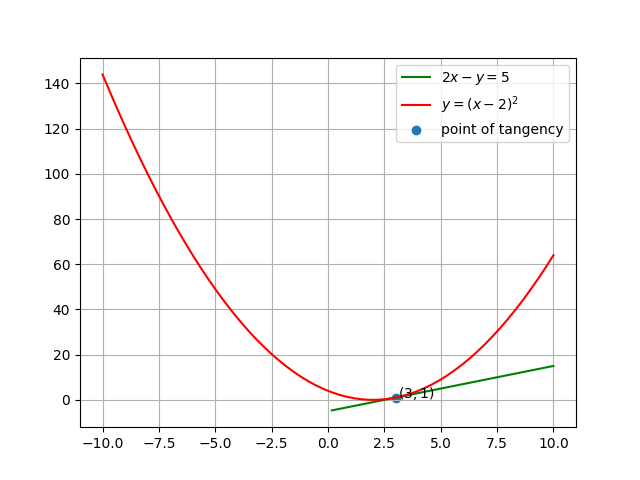
\includegraphics[width=\columnwidth]{plot.png}
%          \caption{Plot of the triangle}
%          \label{plot}
% \end{figure}
$\therefore$ Average power is :
\begin{align}
    \frac{1}{T}\int_{0}^{T}\lvert x(t)\rvert^2\,dt = \sum_{k=-3}^{3}\lvert a_k\rvert^2
\end{align}
\begin{align}
    P_{avg} &= 9+4+1+4+1+4+9\\
    P_{avg} &= 32
\end{align}
\begin{figure}[!h]
         \centering
         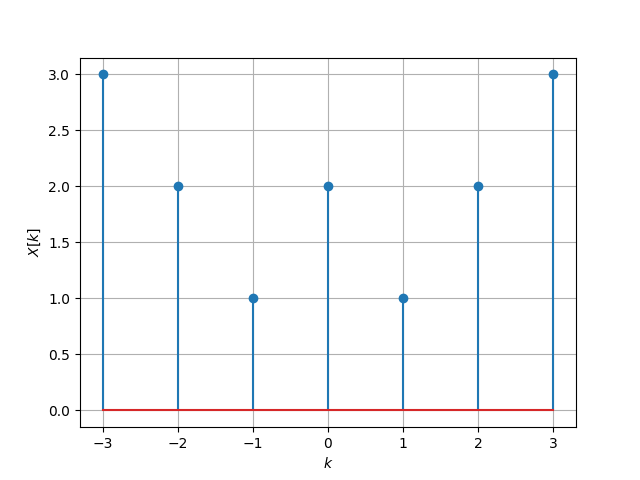
\includegraphics[width=\columnwidth]{plot_X[k].png}
         \caption{Plot of $X[k]$}
         \label{plot}
\end{figure}
\begin{figure}[!h]
         \centering
         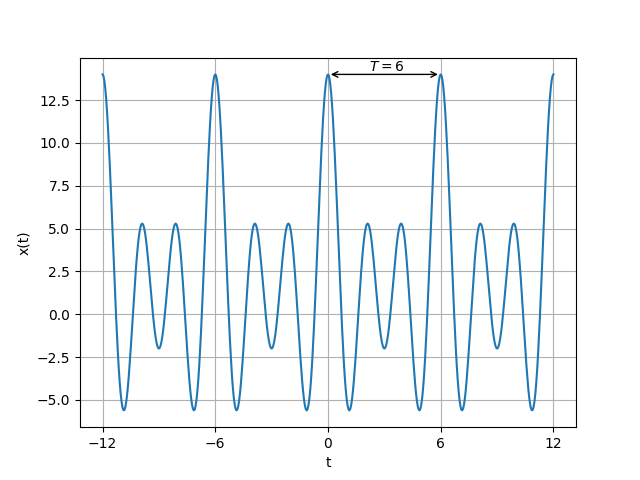
\includegraphics[width=\columnwidth]{plot_x(t).png}
         \caption{Plot of $x(t)$}
         \label{plot}
\end{figure}
\end{document}
